\documentclass[11pt,a4paper]{article}
\usepackage[margin=2.4cm]{geometry}
\usepackage{graphicx}
\usepackage{amsmath}
\usepackage{xcolor}
\usepackage[colorlinks=true,linkcolor=blue!50!black,urlcolor=blue!50!black]{hyperref}
\graphicspath{{figs/}}

\newcommand{\He}[1]{$^{#1}$He}
\newcommand{\snp}{\sigma_{np}}
\newcommand{\sng}{\sigma_{n\gamma}}

\title{\vspace{-1.2cm}
  {\Large\bfseries Thermal-neutron statistics for X17 production at n\_TOF EAR2}\\[2mm]
  {\large What $4\times10^{8}$ fully simulated neutrons say about the
   sub-keV rate tables}}
\author{Dylan Neff}
\date{11 June 2026 \\[2mm]
  {\small\itshape Internal note --- informal. Drafted by Claude (Anthropic AI
  assistant) under D.~Neff's direction; \\ simulation, numbers and text
  reviewed by D.~Neff.}\\[1mm]
  {\small\color{red!60!black} PRELIMINARY: based on 40 of 100 run-B jobs
  ($4\times10^{8}$ of $10^{9}$ neutrons); \\ remaining statistics in
  production, no qualitative change expected.}}

\begin{document}
\maketitle

%=============================================================================
\section*{Part I --- Summary}

\subsection*{The question}
The X17 search at EAR2 produces its signal through radiative neutron capture:
a slow neutron absorbed by \He{3} forms \He{4}$^{*}$ at 20.6\,MeV, and that
de-excitation is the only doorway to X17 (or to the internal-pair background,
IPC). The expected event rate per proton pulse therefore scales directly with
the number of \emph{radiative} captures per pulse. The collaboration rate
table (\texttt{calculation\_tables/results\_3He}) quotes
$1.2\times10^{-2}$~IPC/pulse from neutrons below 1\,keV --- the number that
anchored the $3.0\sigma$/30-day sensitivity projection.

\subsection*{The problem}
That table computes the radiative-capture probability as
(target thickness)\,$\times$\,(cross-section), which silently assumes neutrons
fly through the gas undisturbed. They do not. At thermal energy the
competing \He{3}(n,p)t reaction gives a neutron a mean free path of
$\sim$0.1\,mm in a 30\,mm gas column: \textbf{the gas is opaque}. Every
sub-keV neutron is absorbed regardless of the gas thickness, so the rare
radiative branch cannot exceed its share of the total,
$\sng/\snp = 1.0\times10^{-8}$ per absorbed neutron --- no matter how much
gas is added. The thin-target formula overshoots this ceiling by a factor
equal to the gas opacity: $\times$8 to $\times$200 depending on energy.

\subsection*{What we did}
Run~B of the Geant4 campaign fired $10^{9}$ neutrons (this draft: the first
validated $4\times10^{8}$) at the full STEP-derived capsule geometry, with
energies drawn from the evaluated EAR2 flux and transverse positions from the
energy-dependent beam profile, using high-precision neutron data (G4NDL).
Self-shielding, scattering, beam halo and geometry are then automatic --- no
analytic assumption. Every neutron's terminal interaction (volume, process,
position, energy) was recorded.

\subsection*{The answer}
\begin{center}
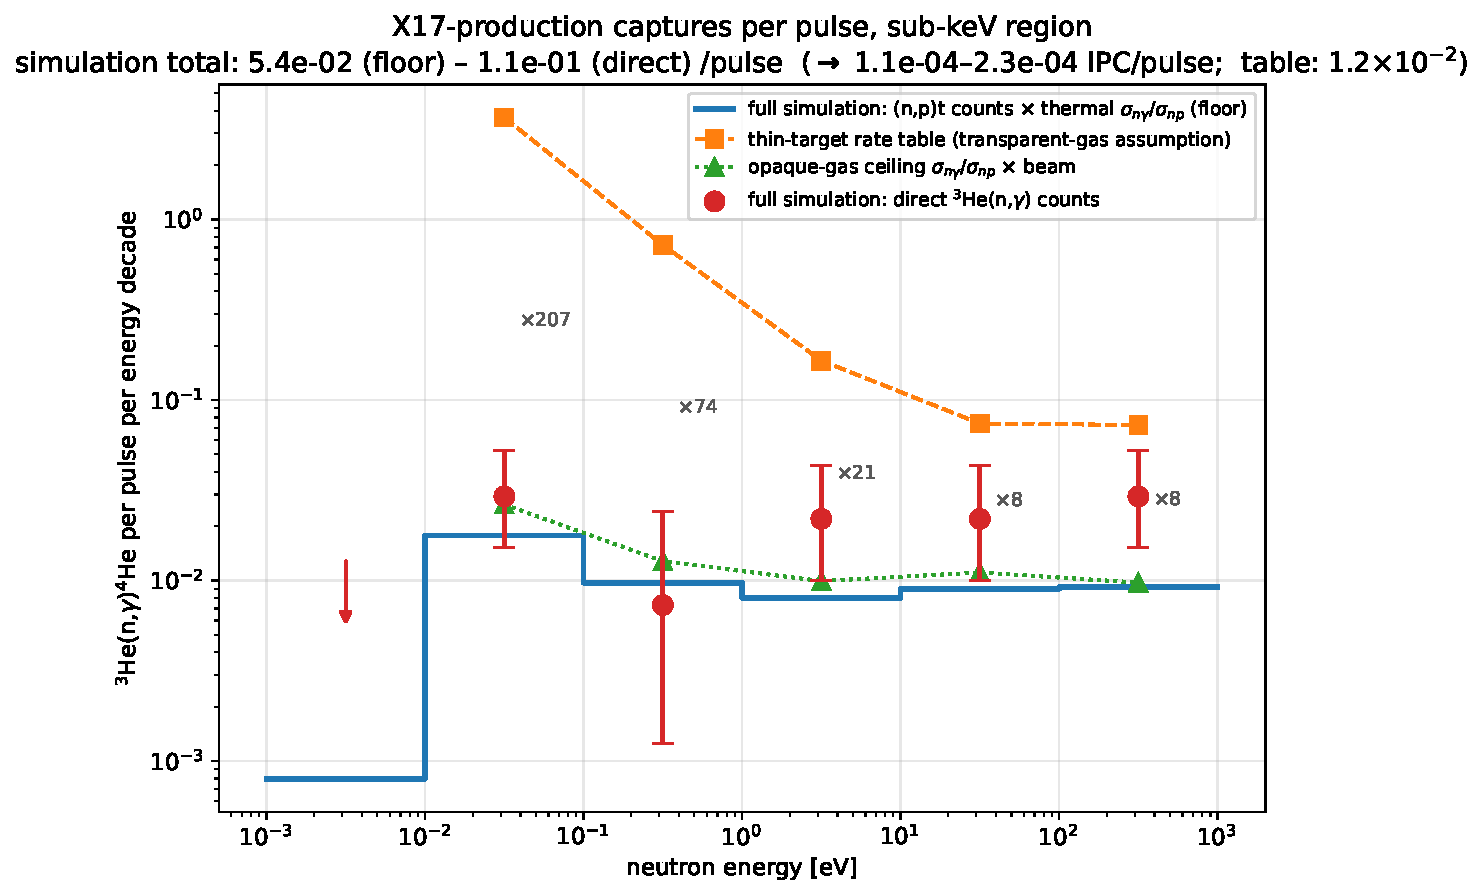
\includegraphics[width=0.92\textwidth]{fig_money.pdf}
\end{center}

\noindent The full simulation (blue curve, with the four directly observed
radiative captures as red points) lands on the opaque-gas ceiling (green) and
confirms the rate table (orange) is too optimistic by $\times$8--200 per
decade. Folding in the beam spectrum:

\begin{center}
\begin{tabular}{lcc}
\hline
 & rate table & full simulation \\
\hline
radiative captures / pulse ($E_n<1$\,keV) & $5.8$ & $5.4\times10^{-2}$ \\
IPC / pulse                               & $1.21\times10^{-2}$ & $1.14\times10^{-4}$ \\
X17 / pulse (2.5\% assumed)               & ---                & $1.4\times10^{-3}$ \\
\hline
\end{tabular}
\end{center}

\noindent\textbf{The sub-keV statistics are a factor $\sim$106 below the
table.} If the sensitivity projection is anchored to the sub-keV rows, the
$3.0\sigma$/30\,d becomes $\sim$0.3$\sigma$/30\,d. The physical rate is not
gone, however: above $\sim$100\,keV the gas really is thin and the table is
valid there; those rows carry $\sim$98\% of the total radiative captures.
The likely conclusion is that \textbf{the analysis region of interest must
move to the 0.1--10\,MeV region}, which changes the generator kinematics and
the gamma-flash/TOF situation --- to be discussed with Alberto (run B-full,
1\,meV--100\,MeV, is already on disk for this).

%=============================================================================
\clearpage
\section*{Part II --- The full story, from the beginning}

\section{What can happen when a slow neutron meets \He{3}}

When the neutron is absorbed, the compound nucleus \He{4}$^{*}$ holds
20.6\,MeV of excitation energy. It almost always sheds it by breaking into a
proton and a triton --- a quiet outcome that deposits heat in the gas and
produces no high-energy photon. About once in $10^{8}$ absorptions it instead
de-excites electromagnetically, and only this branch can produce a real
20.6\,MeV photon, an internal e$^+$e$^-$ pair, or --- if it exists --- the
X17 boson. Counting X17 statistics is therefore exactly the business of
counting these rare radiative captures.

\begin{center}
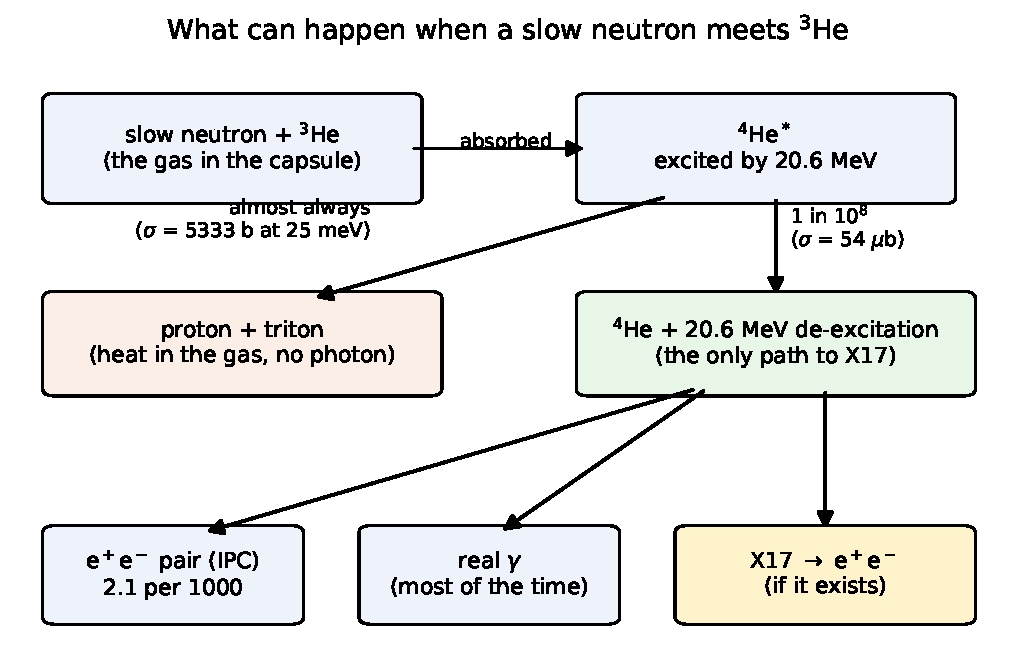
\includegraphics[width=0.85\textwidth]{fig_reaction_tree.pdf}
\end{center}

The two relevant cross-sections at thermal energy (25\,meV):
breakup $\snp = 5333$\,b, radiative $\sng = 54\,\mu$b. Both fall as
$1/v$ with neutron speed, so their ratio,
\begin{equation}
  \frac{\sng}{\snp} = \frac{54\times10^{-6}}{5333}
  = 1.0\times10^{-8},
  \label{eq:ratio}
\end{equation}
is essentially constant across the whole sub-keV region. Keep this number in
mind --- it is the punchline of the entire note.

\section{What the beam delivers}

EAR2 delivers $7.31\times10^{6}$ neutrons per proton pulse below 1\,keV
(evaluated Phase-3 flux). The beam is not a pencil: its transverse size
grows toward low energies, while the capsule bore is only 20\,mm across, so
an energy-dependent fraction of the beam misses the gas entirely or hits the
thick aluminium shoulder instead. The simulation samples both the energy
spectrum and this energy-dependent footprint, so all acceptance effects are
folded in from the start.

\begin{center}
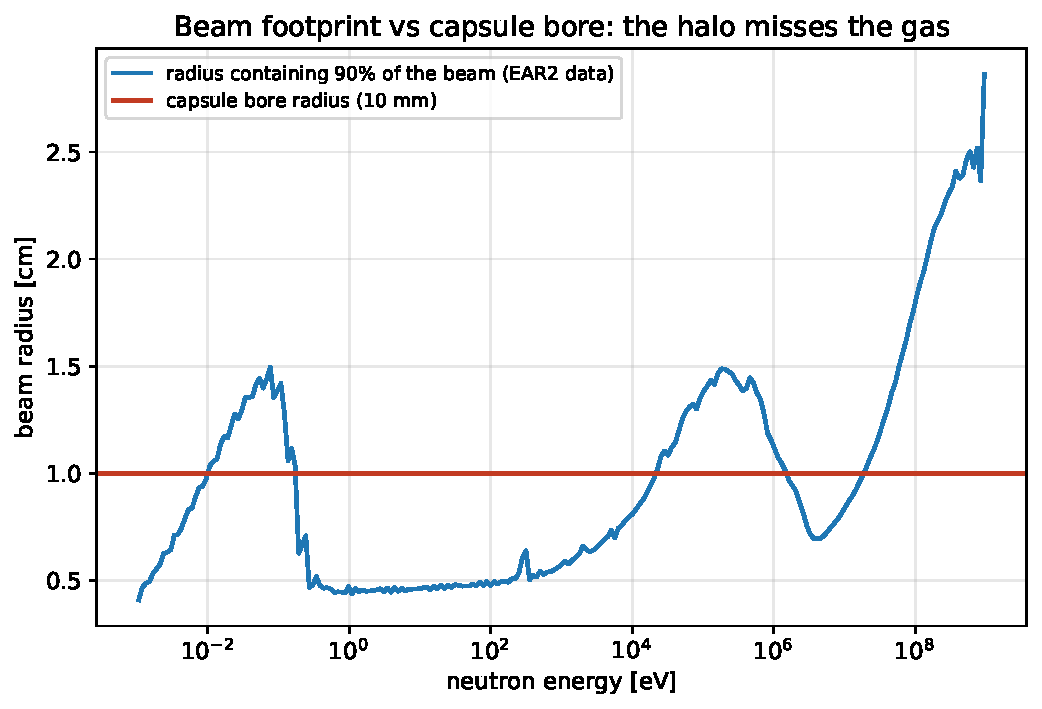
\includegraphics[width=0.78\textwidth]{fig_footprint.pdf}
\end{center}

\begin{center}
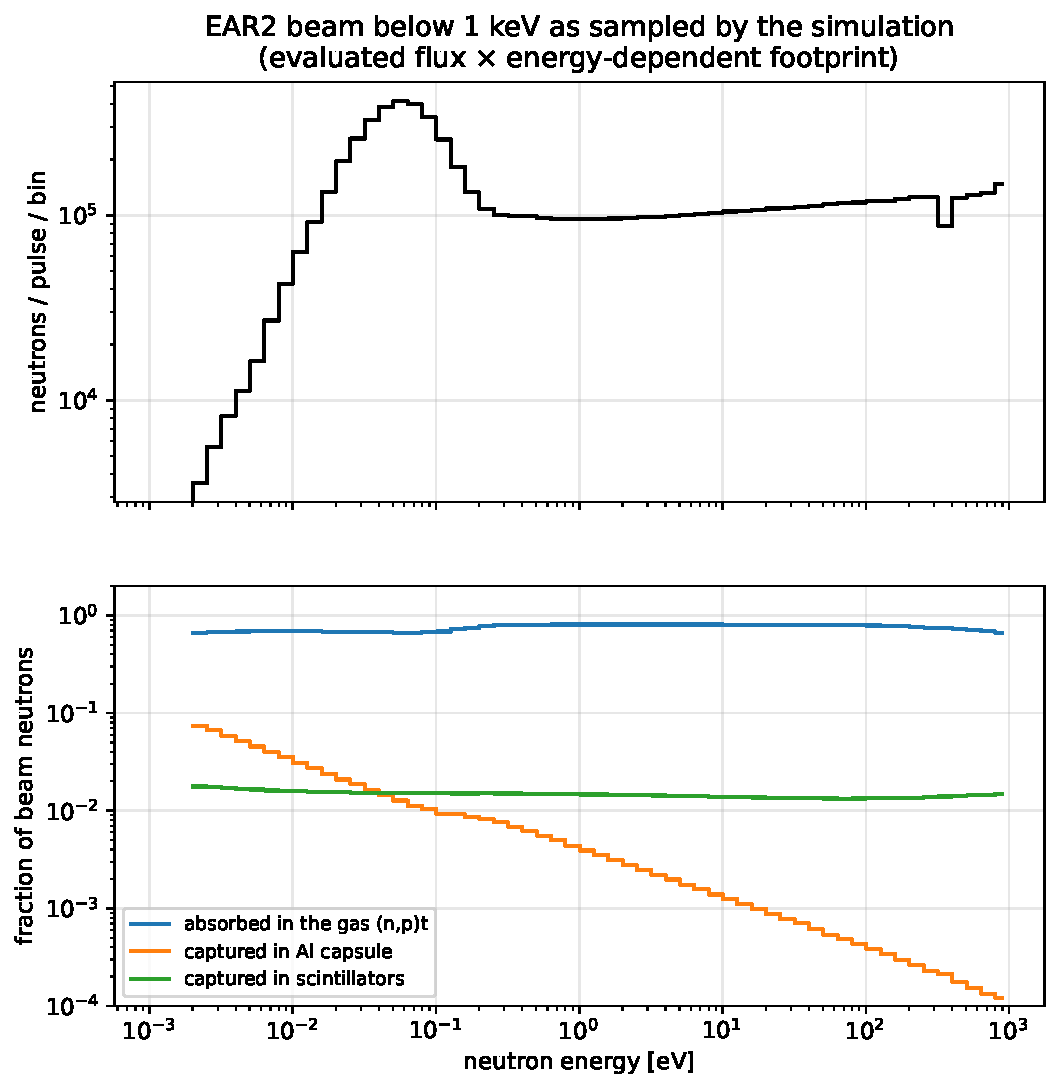
\includegraphics[width=0.8\textwidth]{fig_beam_fates.pdf}
\end{center}

\noindent In numbers, for the sub-keV beam: 73.6\% of all beam neutrons are
absorbed in the gas, 23.9\% leave the world without interacting (mostly
footprint tail outside the bore), and the remainder is captured in
surrounding material --- of which more in Sec.~\ref{sec:walls}.

\section{The core issue: the gas is a black absorber, not a thin foil}
\label{sec:opaque}

\begin{center}
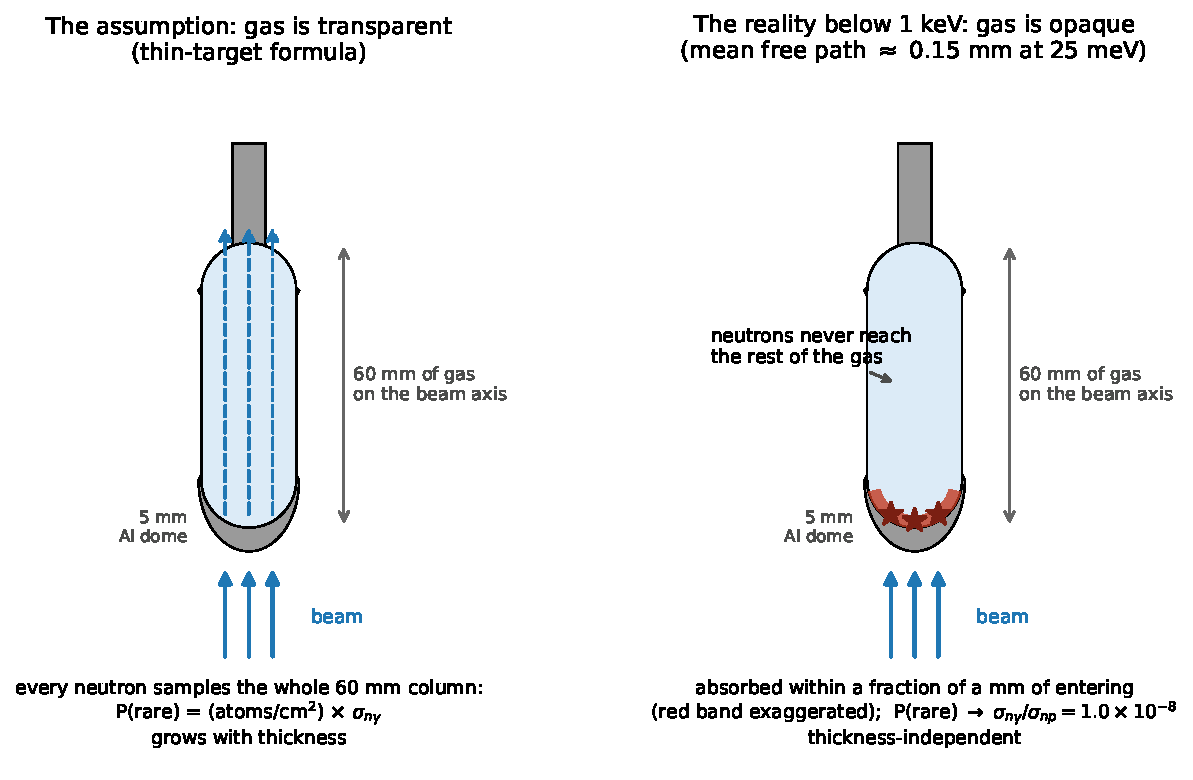
\includegraphics[width=\textwidth]{fig_opaque_cartoon.pdf}
\end{center}

The rate table computes, for each energy bin,
\begin{equation}
  P_{\text{rad}} = n L \cdot \sng(E),
  \label{eq:thin}
\end{equation}
with $nL = 3.16\times10^{-2}$\,atoms/b the gas column. This is the standard
\emph{thin-target} formula and it is correct \emph{only} when the neutron
actually traverses the full column, i.e.\ when $nL\,\snp \ll 1$. At 25\,meV,
however, $nL\,\snp \approx 150$: a neutron penetrates a fraction of a
millimetre before being absorbed. In that regime the probability that the
absorption is radiative saturates at the branching ratio:
\begin{equation}
  P_{\text{rad}} \;\longrightarrow\; \frac{\sng}{\snp} = 1.0\times10^{-8}
  \qquad \text{(independent of } L\text{)}.
  \label{eq:cap}
\end{equation}
Dividing Eq.~\eqref{eq:thin} by Eq.~\eqref{eq:cap} shows the thin-target
formula overshoots by exactly the opacity $nL\,\snp$ --- the factor 150 at
thermal, falling to $\sim$7 at 1\,keV. Adding more gas, or pressurising
further, gains nothing below 1\,keV: every neutron is already absorbed, and
the radiative branch can only ever win its fixed share.

\section{What the full simulation adds}

The cartoon argument above is one-dimensional. The real situation has a
domed entrance window, a beam wider than the bore, elastic scattering that
can bounce neutrons around, resonances in the surrounding materials, and a
gas column whose length depends on where the neutron enters. Geant4 with
high-precision neutron data (G4NDL) transports every neutron through the
actual STEP-derived geometry and lets nature take its course. The simulation
records, for each of the $4\times10^{8}$ neutrons in this draft, where its
track ended, by which process, and at what energy --- so the capture
accounting is exact, including all geometry and transport effects.

\section{The evidence}

\subsection{Self-shielding, observed directly}
If the opaque-gas picture is right, thermal neutrons must pile up at the
entrance face of the gas while keV neutrons penetrate deeper. That is
exactly what the absorption-depth distribution shows:

\begin{center}
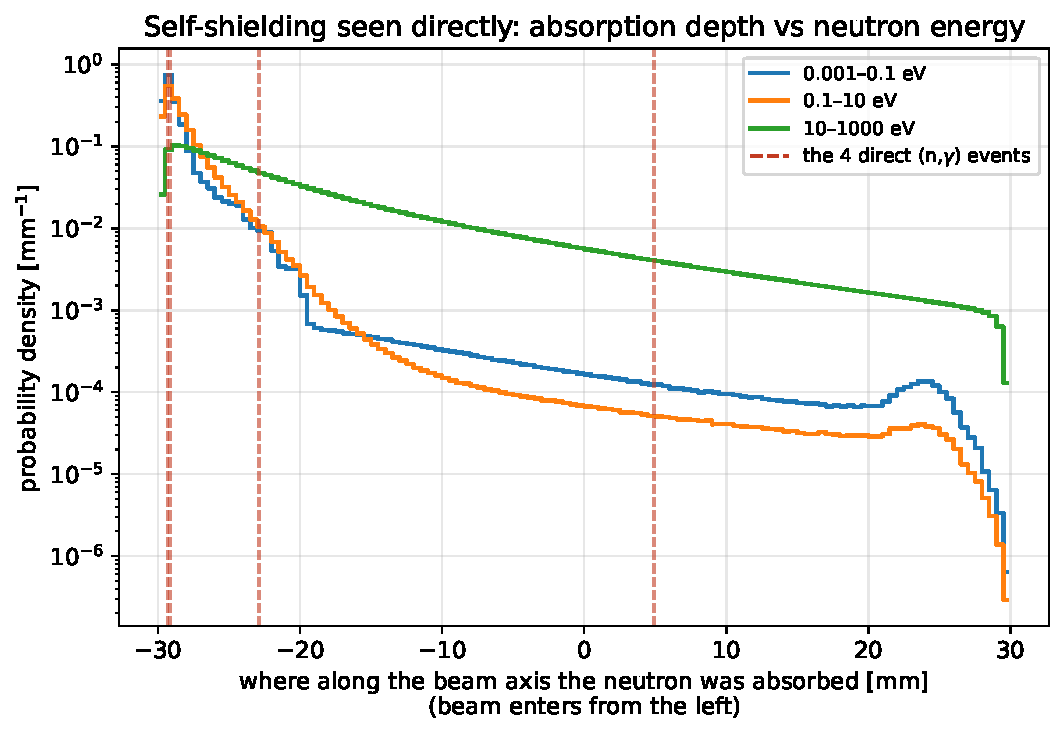
\includegraphics[width=0.8\textwidth]{fig_depth.pdf}
\end{center}

\noindent Below 0.1\,eV the absorption depth is a sliver at the entrance; by
0.1--1\,keV it spreads through the column. The four directly observed
radiative captures (dashed lines) follow the same pattern: the two thermal
ones sit within a millimetre of the entrance window, the two at
$\sim$500\,eV are distributed through the gas.

\subsection{The rate, measured three ways}
The headline figure (Part I) compares, per energy decade:
\begin{enumerate}
  \item \textbf{Direct counts}: four \He{3}(n,$\gamma$) events in
        $4\times10^{8}$ neutrons $\Rightarrow$
        $(1.0^{+0.8}_{-0.5})\times10^{-8}$ per beam neutron.
  \item \textbf{High-statistics proxy}: $2.94\times10^{8}$ observed (n,p)t
        absorptions multiplied by the branching ratio of
        Eq.~\eqref{eq:ratio} --- statistically exact in the opaque regime,
        since every absorbed neutron had the same $10^{-8}$ chance of taking
        the radiative exit instead.
  \item \textbf{The analytic ceiling}: Eq.~\eqref{eq:cap} times the beam.
\end{enumerate}
All three agree. The rate table exceeds them by $\times$207 (thermal decade)
down to $\times$8 (100\,eV--1\,keV); the row-by-row comparison is in
Appendix~A. As a by-product the agreement of (1) and (2) confirms that the
G4NDL nuclear data contain the radiative branch at the right strength ---
the ratio test gives
$N_{n\gamma}/N_{np} = 1.4^{+1.1}_{-0.7}\times10^{-8}$ against the expected
$1.0\times10^{-8}$.

\subsection{From captures to X17 per pulse}
\begin{center}
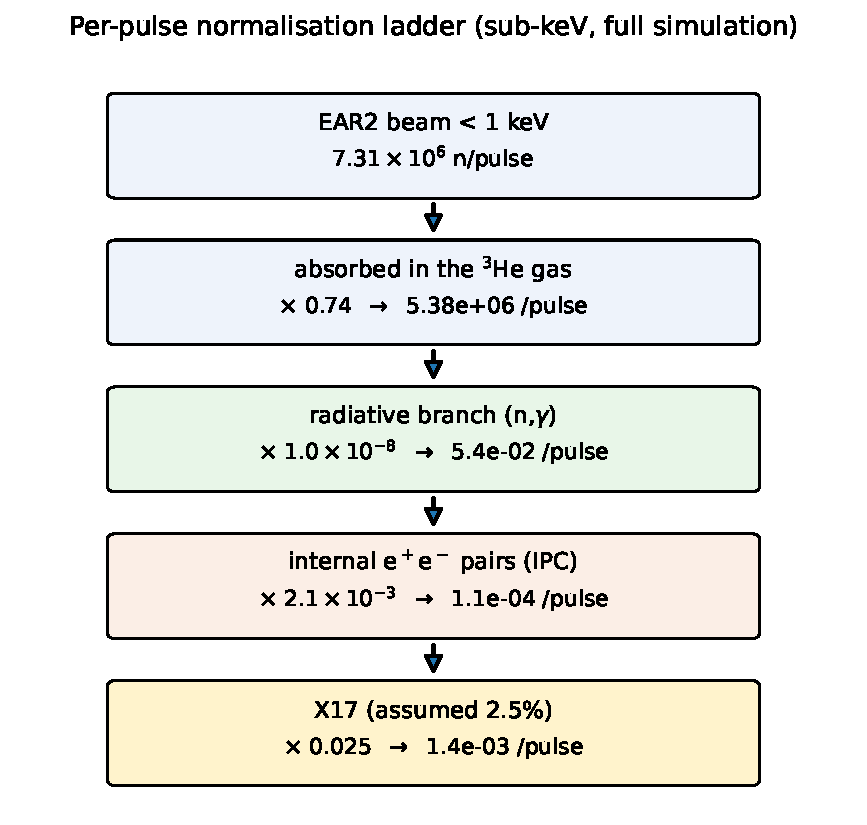
\includegraphics[width=0.62\textwidth]{fig_ladder.pdf}
\end{center}

\section{Where the neutrons actually end up}
\label{sec:walls}

A secondary deliverable of run~B, relevant for backgrounds rather than
signal statistics. Per beam neutron below 1\,keV:

\begin{center}
\begin{tabular}{lll}
\hline
fate & per beam neutron & comment \\
\hline
\He{3}(n,p)t in gas        & $7.4\times10^{-1}$ & signal-region heat, no photons \\
escapes world              & $2.4\times10^{-1}$ & footprint tail \\
capture in Al capsule      & $8.0\times10^{-3}$ & 7.7\,MeV $\gamma$ cascades near target \\
capture in liquid scint.   & $1.2\times10^{-2}$ & 2.2\,MeV $\gamma$ born \emph{inside} calorimeter \\
capture in plastic scint.  & $2.2\times10^{-3}$ & trigger + back layers \\
capture in CFRP/PCB/mesh   & $\sim1.5\times10^{-3}$ & distributed \\
\He{3}(n,$\gamma$)         & $1.0\times10^{-8}$ & the X17 channel \\
\hline
\end{tabular}
\end{center}

\noindent Two observations. First, the aluminium capture rate is $\sim$60
times the old flat-cap toy estimate --- the STEP capsule's domed tip and
thick shoulder put far more Al in the beam. Second, and not in any toy so
far: \textbf{hydrogen capture in the liquid scintillator is the largest
single capture channel outside the gas}, and its 2.22\,MeV photon is born
inside the calorimeter itself. Both feed the wall-background simulation
(run~C) via the capture-vertex library.

\section{What this means for the experiment}

\begin{itemize}
  \item \textbf{Sub-keV ROI}: $1.1\times10^{-4}$ IPC/pulse and
        $1.4\times10^{-3}$ X17/pulse (at the assumed 2.5\%) --- a factor
        $\sim$106 below the table. A thermal-only analysis cannot reach
        the projected significance; scaled naively, $3.0\sigma \to
        0.3\sigma$ over 30 days.
  \item \textbf{The MeV region}: above $\sim$100\,keV the gas opacity drops
        below 5\% and the thin-target rows of the table become valid; they
        carry $\sim$98\% of all radiative captures. The commented-out
        0.2--2\,MeV row ($5.2\times10^{-2}$ IPC/pulse) looks like the right
        anchor. Moving there requires (a) energy-dependent pair kinematics
        in the generator ($E^{*} \approx 20.58\,\text{MeV} + \tfrac34 E_n$
        plus a centre-of-mass boost), and (b) an assessment of the gamma
        flash and TOF window at $\mu$s timescales. Run~B-full
        (1\,meV--100\,MeV) is on disk to quantify the capture budget there.
  \item \textbf{For discussion with Alberto}: which rows anchored the
        sensitivity; the provenance of the IPC coefficient
        ($2.1\times10^{-3}$ --- multipolarity, E0 contribution); and the
        capsule-geometry update (the table assumed a 4\,cm sphere).
\end{itemize}

\section*{Caveats}
\begin{itemize}
  \item Statistics: this draft uses 40 of 100 run-B jobs; the remaining
        60 are in production (quota-related corruption, resubmitted).
        All conclusions rest on the $2.9\times10^{8}$-event (n,p) sample
        and are insensitive to the final factor 2.5.
  \item The G4NDL \He{3}(n,$\gamma$) strength is validated here only at the
        $\sim$50\% level (4 events); the branching-ratio argument does not
        depend on it.
  \item Room-return neutrons and upstream beamline structures are not in
        the simulation; they affect backgrounds, not the signal-rate
        conclusion.
  \item The simulated radial profile and flux are the evaluated Phase-3
        EAR2 ones; if the beam group provides updated halo measurements,
        the footprint losses (24\% escape) could shift.
\end{itemize}

%=============================================================================
\clearpage
\appendix
\section{Row-by-row comparison with the rate table}

Radiative captures per \emph{beam} neutron, per energy decade. ``Table''
reproduces \texttt{results\_3He} (thin-target); ``ceiling'' is
Eq.~\eqref{eq:cap} corrected for the (n,p) opacity within the decade;
``simulation'' is the (n,p)$\times$BR measurement from $4\times10^{8}$
neutrons (statistical errors negligible); ``direct'' are the raw
\He{3}(n,$\gamma$) counts.

\begin{center}
\begin{tabular}{lccccc}
\hline
$E_n$ range & table & simulation & table/sim & ceiling & direct counts \\
\hline
1--10\,meV      & ---                 & $6.9\times10^{-9}$ & ---  & ---                & 0 \\
10--100\,meV    & $1.41\times10^{-6}$ & $6.8\times10^{-9}$ & 207  & $1.01\times10^{-8}$ & 2 \\
0.1--1\,eV      & $5.71\times10^{-7}$ & $7.7\times10^{-9}$ & 74   & $1.01\times10^{-8}$ & 0 \\
1--10\,eV       & $1.68\times10^{-7}$ & $8.2\times10^{-9}$ & 21   & $1.01\times10^{-8}$ & 0 \\
10--100\,eV     & $6.69\times10^{-8}$ & $8.1\times10^{-9}$ & 8.3  & $1.00\times10^{-8}$ & 0 \\
0.1--1\,keV     & $5.90\times10^{-8}$ & $7.5\times10^{-9}$ & 7.9  & $7.9\times10^{-9}$  & 2 \\
\hline
\end{tabular}
\end{center}

\noindent The simulation sits 20--30\% \emph{below} the ceiling because the
ceiling assumes every beam neutron is absorbed in the gas, while in reality
67--81\% are (footprint tail and window transmission) --- visible in the
(n,p) column of the per-decade scan output. Flux-weighted over the full
sub-keV window the table gives $1.21\times10^{-2}$ IPC/pulse against the
simulation's $1.14\times10^{-4}$: \textbf{factor 106}.

\section{The four direct events, and provenance}

\begin{center}
\begin{tabular}{cc}
\hline
$E_n$ & absorption depth along beam axis \\
\hline
12.4\,meV & $-29.2$\,mm (at the entrance face) \\
13.5\,meV & $-29.3$\,mm (at the entrance face) \\
478\,eV   & $+4.9$\,mm (mid-column) \\
519\,eV   & $-22.9$\,mm \\
\hline
\end{tabular}
\end{center}

\noindent Data: run B sub-keV, 40 validated jobs
($4\times10^{8}$ neutrons), \\
\texttt{/eos/experiment/ntof/data/x17/full\_sim/neutrons\_subkev/}. \\
Scan: \texttt{scripts/analyze\_thermal\_captures.py} $\to$
\texttt{thermal\_captures\_subkev\_prelim.npz/json}. \\
Figures: \texttt{scripts/make\_thermal\_report\_figures.py}.
Repository: \texttt{MX17\_Full\_Geant}, branch \texttt{main}.

\end{document}
